%% 第一章--chapter1.tex
\chapter{绪论}
\section{字体}
\subsection{字体配置}
模板配置了两种字库,以 \opt{fontset = windows} 为例:
\begin{enumerate}
	\item 中文:主字体(衬线字体)为中易宋体,无衬线字体族为中易黑体,%
	且二者均可加粗为对应的伪粗体;《规范》中未规定的楷体和仿宋均为 \pkg{ctex} 宏集的预设,为避免格式审查问题,应当减少使用;
	\item 西文:除英文摘要的关键词使用中易黑体、除公式中的西文(数字、字母等)使用特殊字体,其它一律使用 Times New Roman;
	\item 公式:模板会根据实际字体安装情况,选择 $LibertinusMath$ 字体或使用 \LaTeX\ 的默认字体。
\end{enumerate}

\subsection{中文字体命令及对应西文示例}
\begin{enumerate}
	\item 宋体:北京化工大学 BUCT 1958 或 \textrm{北京化工大学 BUCT 1958}
	\item 粗宋体:{\bfsong 北京化工大学 BUCT 1958} 或 \emph{北京化工大学 BUCT 1958}
	\item 黑体:{\heiti 北京化工大学 BUCT 1958} 或 \textsf{北京化工大学 BUCT 1958}
	\item 粗黑体:{\bfhei 北京化工大学 BUCT 1958} 或 \textsf{\bfseries 北京化工大学 BUCT 1958}
	\item 仿宋:{\ttfamily 北京化工大学 BUCT 1958} 或 \texttt{北京化工大学 BUCT 1958}
	\item 斜体:{\itshape 北京化工大学 BUCT 1958} 或 \textit{北京化工大学 BUCT 1958}
\end{enumerate}

\section{浮动体}
% 一些文字用来充版面。摘自 https://github.com/chinese-poetry/chinese-poetry
六王毕,四海一,蜀山兀,阿房出。覆压三百余里,隔离天日。骊山北构而西折,直走咸阳。
二川溶溶,流入宫墙。五步一楼,十步一阁;廊腰缦回,檐牙高啄;各抱地势,钩心斗角。
盘盘焉,囷囷焉,蜂房水涡,矗不知其几千万落。长桥卧波,未云何龙?复道行空,不霁何虹?
高低冥迷,不知西东。歌台暖响,春光融融;舞殿冷袖,风雨凄凄。一日之内,一宫之间,而气候不齐。

妃嫔媵嫱,王子皇孙,辞楼下殿,辇来于秦,朝歌夜弦,为秦宫人。明星荧荧,开妆镜也;
绿云扰扰,梳晓鬟也;渭流涨腻,弃脂水也;烟斜雾横,焚椒兰也。雷霆乍惊,宫车过也;
辘辘远听,杳不知其所之也。一肌一容,尽态极妍,缦立远视,而望幸焉。有不见者,三十六年。
燕赵之收藏,韩魏之经营,齐楚之精英,几世几年,剽掠其人,倚叠如山。一旦不能有,输来其间。
鼎铛玉石,金块珠砾,弃掷逦迤,秦人视之,亦不甚惜。

\subsection{插图}\label{subsec:fig}

一般的图片插入使用 \env{figure} 环境。
一张普普通通的插图参见图~\ref{fig:a-single-image}。

\begin{figure}[H]
	\centering
	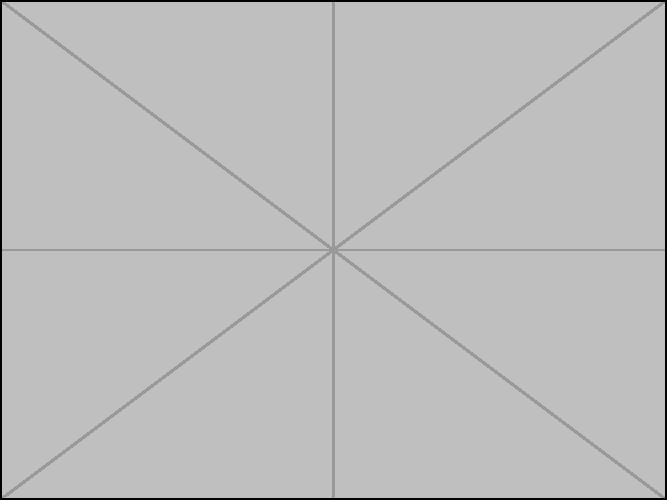
\includegraphics[width=0.3\textwidth]{image-plain.pdf}
	\caption{一张插图。加上参数 [H] 固定图片位置,禁止“浮动”}\label{fig:a-single-image}
\end{figure}

嗟乎!一人之心,千万人之心也。秦爱纷奢,人亦念其家。奈何取之尽锱铢,用之如泥沙!
使负栋之柱,多于南亩之农夫;架梁之椽,多于机上之工女;钉头磷磷,多于在庾之粟粒;
瓦缝参差,多于周身之帛缕;直栏横槛,多于九土之城郭;管弦呕哑,多于市人之言语。
使天下之人,不敢言而敢怒。独夫之心,日益骄固。戍卒叫,函谷举,楚人一炬,可怜焦土!

至于图片的并排,如果只需为组图写一个图注,可在一个 \env{figure} 环境中多次使用 \cs{includegraphics} 命令(可根据需要在插图之间加入空白)。两张并排的图片参见图~\ref{fig:abreast-image}。

\begin{figure}[htbp]
	\centering
	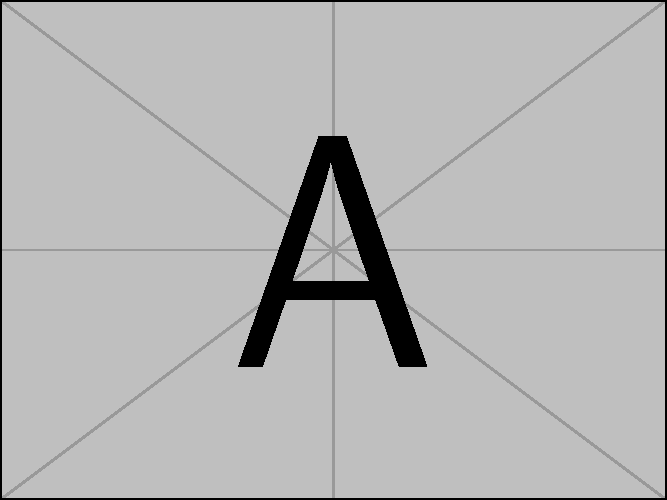
\includegraphics[width=0.3\textwidth]{image-a.pdf}
	\hspace{1cm}
	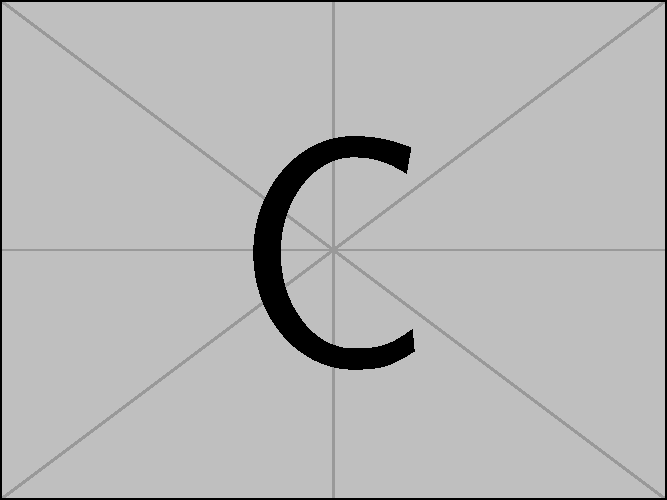
\includegraphics[width=0.3\textwidth]{image-c.pdf}
	\caption{并排的插图,这适合无需在每一张图下写图注的情况。}\label{fig:abreast-image}
\end{figure}

呜呼!灭六国者六国也,非秦也;族秦者秦也,非天下也。嗟乎!使六国各爱其人,则足以拒秦;
使秦复爱六国之人,则递三世可至万世而为君,谁得而族灭也?秦人不暇自哀,而后人哀之;
后人哀之而不鉴之,亦使后人而复哀后人也。

梁惠王曰:“寡人之于国也,尽心焉耳矣。河内凶,则移其民于河东,移其粟于河内;河东凶亦然。
察邻国之政,无如寡人之用心者。邻国之民不加少,寡人之民不加多,何也?

但如果需要在每一个子图下写上图注(或需要对子图标序),可使用 \cs{subcaptionbox} 命令。
一张子图见图~\ref{subfig:abreast-image-a},又一张子图见图~~\ref{subfig:abreast-image-c},这两张并排起来的组图见图~\ref{fig:abreast-image-a-c}。

\begin{figure}[htbp]
	\centering
	\subcaptionbox{这是一张图片。\label{subfig:abreast-image-a}}
	{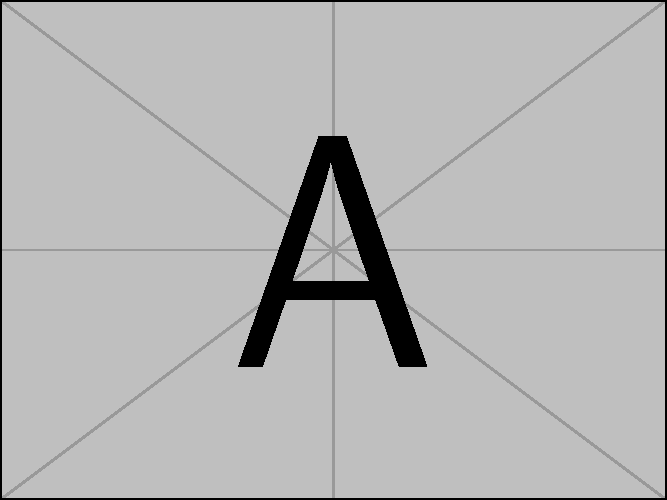
\includegraphics[height = 5cm]{image-a.pdf}}
	\hspace{1cm}
	\subcaptionbox{这又是一张图片。\label{subfig:abreast-image-c}}
	{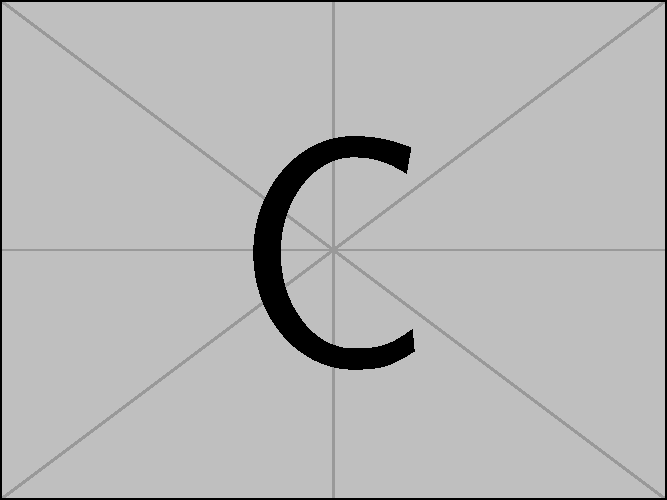
\includegraphics[angle = 90, height = 5cm]{image-c.pdf}}
	\caption{并排的插图,这适合每一张图写一个图注的情况。}\label{fig:abreast-image-a-c}
\end{figure}

孟子对曰:“王好战,请以战喻。填然鼓之,兵刃既接,弃甲曳兵而走。或百步而后止,
或五十步而后止。以五十步笑百步,则何如?”曰:“不可,直不百步耳,是亦走也。”
曰:“王如知此,则无望民之多于邻国也。不违农时,谷不可胜食也;数罟不入洿池,
鱼鳖不可胜食也;斧斤以时入山林,材木不可胜用也。谷与鱼鳖不可胜食,材木不可胜用,
是使民养生丧死无憾也。养生丧死无憾,王道之始也。五亩之宅,树之以桑,五十者可以衣帛矣
。鸡豚狗彘之畜,无失其时,七十者可以食肉矣。百亩之田,勿夺其时,数口之家,可以无饥矣;
谨庠序之教,申之以孝悌之义,颁白者不负戴于道路矣。七十者衣帛食肉,黎民不饥不寒,
然而不王者,未之有也。狗彘食人食而不知检,涂有饿莩而不知发,人死,则曰:‘非我也,
岁也。’是何异于刺人而杀之,曰‘非我也,兵也’?王无罪岁,斯天下之民至焉。”

(机械设计等)设计图纸需要编目。模板新定义了类似 \env{figure} 的 \env{dfigure}环境。
设计图纸的标签与普通插图不同,且计数器相互独立。
对于图纸的编目,可以在主文件以 \cs{listofdesignfigures} 生成独立的目录,或使用
\cs{dcaption}\marg{Caption}命令与主目录合并。
\begin{dfigure}% [H] or [htbp] is also available here.
	\centering
	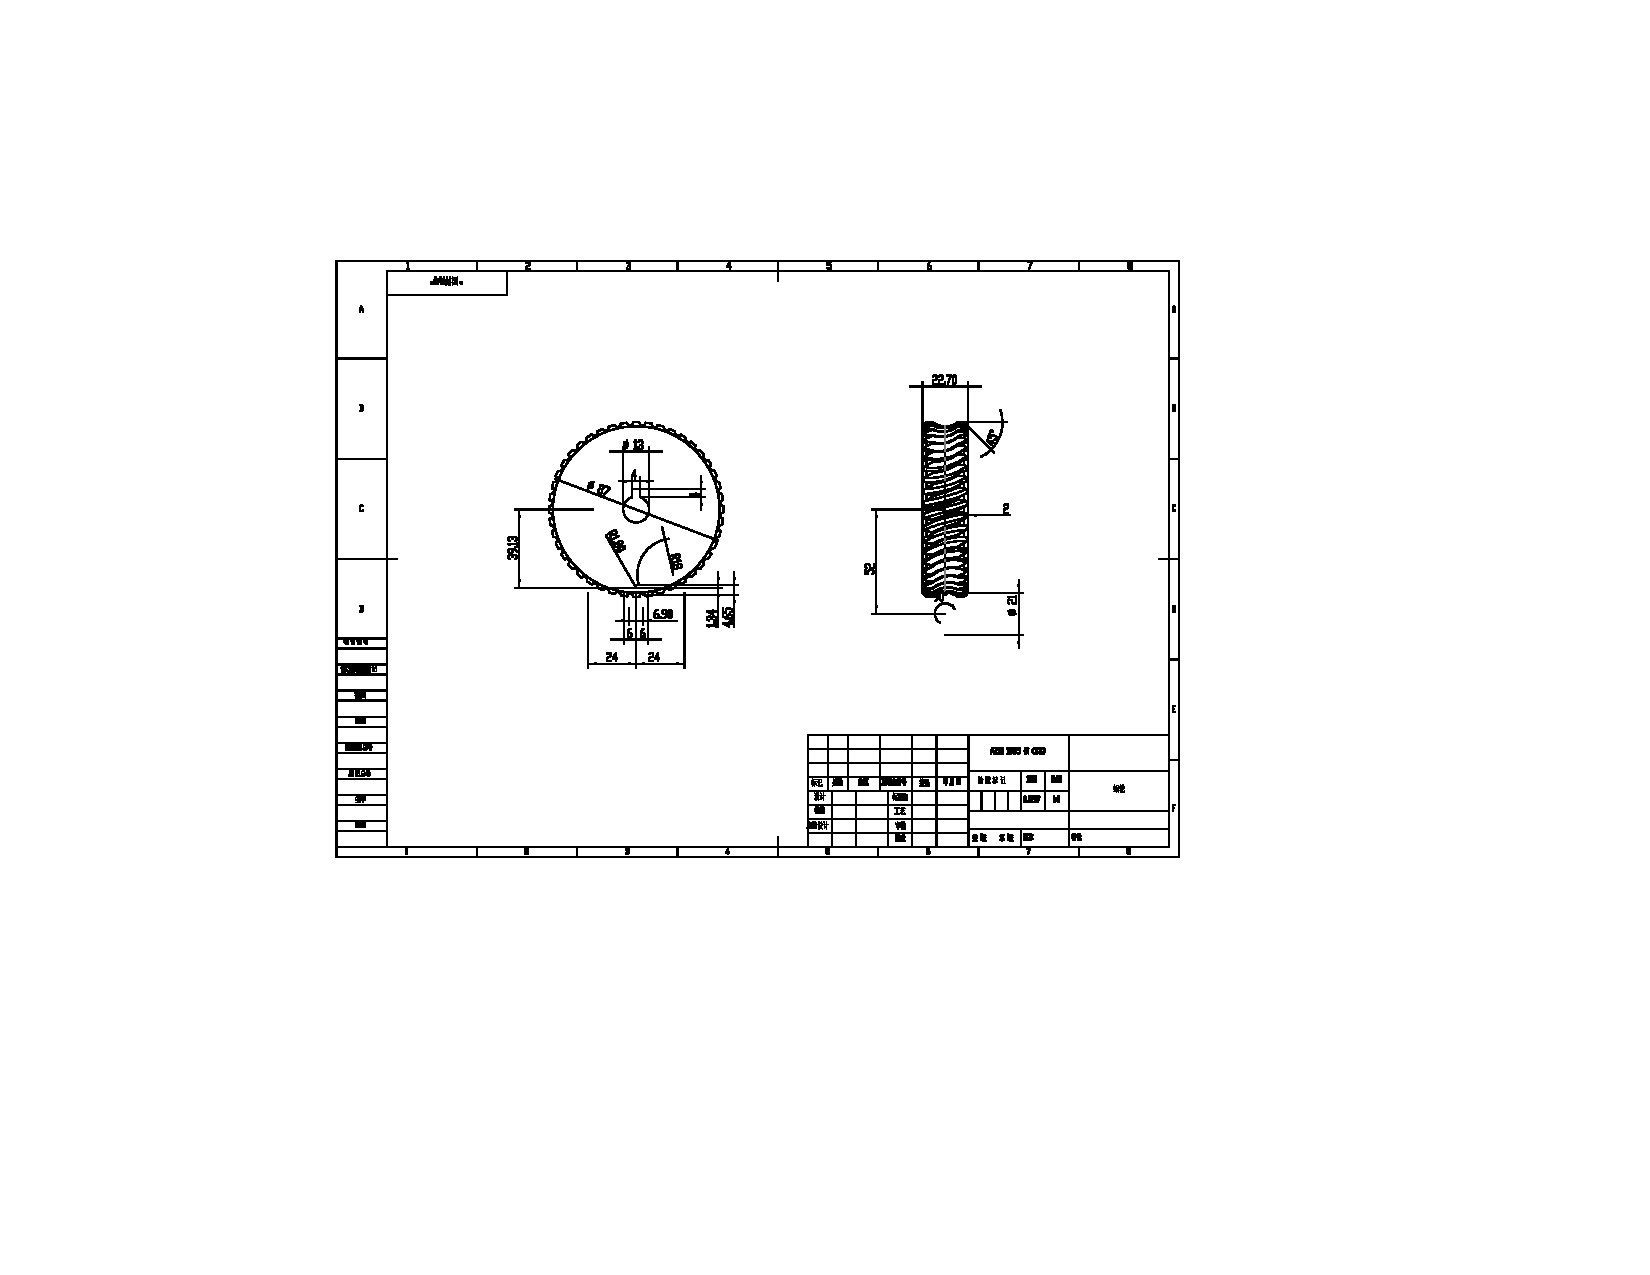
\includegraphics[width = \textwidth]{worm-gear.pdf}
	\caption{设计图纸示例}  % \dcaption{设计图纸示例} % 该命令将其编入主目录。
\end{dfigure}

以上命令适合大部分图片的插入。
但不可否认的是,\LaTeX{}对于图文混排的能力是较弱的,如果希望深入了解,推荐~
\href{https://github.com/WenboSheng/epslatex-cn}{\LaTeXe 插图指南}
(中译本第三版)作为参考资料。


\subsection{表格}\label{subsec:tab}
论文中常用三线表。本模板的组成见表~\ref{tab:mainfile}。

\begin{table}[ht]
	\centering
	\caption{模板的组成}\label{tab:mainfile}
		\begin{tabular}{ll}
			\toprule
			文件(夹)名           & 简述\\
			\midrule
			\file{chapter/}       & 论文各个部分的源文件路径\\
			\file{code/}          & 源代码的路径\\
			\file{figure/}        & 插图的路径\\
			\file{buctthesis.ins} & \textsc{DocStrip} 驱动文件\\
			\file{buctthesis.dtx} & \textsc{DocStrip} 源文件\\
			\file{main.tex}       & 主文件\\
			\file{main.pdf}       & 示例文档\\
			\file{buctthesis.cls} & 模板的文档类文件\\
			\file{thesisbib.bib}  & \BibTeX{}参考文献数据库\\
			\file{mycfg.sty}      & 自定义配置文件\\
			\file{README.md}      & 项目自述文件\\
			\file{buctthesis.pdf} & 写作指南\\
			\bottomrule
		\end{tabular}
\end{table}

北冥有鱼,其名为鲲。鲲之大,不知其几千里也。化而为鸟,其名为鹏。鹏之背,
不知其几千里也,怒而飞,其翼若垂天之云。是鸟也,海运则将徙于南冥。南冥者,
天池也。《齐谐》者,志怪者也。《谐》之言曰:“鹏之徙于南冥也,水击三千里,
抟扶摇而上者九万里,去以六月息者也。”

使用 \cs{hline}命令也能划线,但其线宽固定。关于表格内对齐与常用的命令见表~\ref{tab:tabcmd}。
\begin{table}[H]
	\centering
	\caption{表格命令举例}\label{tab:tabcmd}
	\begin{tabular}{lcrp{5em}@{\extracolsep{3em}}l}
		\hline
		左对齐 & 居中对齐 & 右对齐 & 定宽               & 增加左侧间距\\
		l     & c        &  r    & p\marg{width}  & @\{\cs{extracolsep}\marg{width}\}\\
		\hline
	\end{tabular}
\end{table}

野马也,尘埃也,生物之以息相吹也。
天之苍苍,其正色邪?其远而无所至极邪?其视下也,亦若是则已矣。且夫水之积也不厚,
则其负大舟也无力。覆杯水于坳堂之上,则芥为之舟;置杯焉则胶,水浅而舟大也。
风之积也不厚,则其负大翼也无力。故九万里,则风斯在下矣,而后乃今培风;
背负青天而莫之夭阏者,而后乃今将图南。

另外,三线表生成横线的命令 \cs{toprule}、\cs{midrule}和
\cs{bottomrule}后可以加一个可选参数来实现对线宽的控制,如果不加参数则为默认值;
而\cs{cline}可针对某些表列画上横线。
此外,两个表格也能横向并列排版,如表~\ref{tab:2tab}。

\begin{table}[H]
	\centering
	\caption{这是一个并列排版的示例}
	\label{tab:2tab}
	\begin{tabular}{|c|r|r|}
		\hline
			& \multicolumn{2}{c|}{成绩} \\\cline{2-3}
		姓名 & 语文 & 数学 \\\hline
		张三 & 91 & 92 \\\hline
		\end{tabular}
	\hspace{1cm}
	\begin{tabular}{|c|r|r|}
		\hline
		\multirow{2}*{姓名} & \multicolumn{2}{c|}{成绩} \\ \cline{2-3}
			& 语文          & 数学 \\ \hline
		李四 & 93           & 94 \\ \hline
		\end{tabular}
\end{table}

蜩与学鸠笑之曰:“我决起而飞,抢榆枋而止,时则不至,而控于地而已矣,奚以之九万里而南为?”
适莽苍者,三餐而反,腹犹果然;适百里者宿舂粮,适千里者,三月聚粮。之二虫又何知?
小知不及大知,小年不及大年。奚以知其然也?朝菌不知晦朔,蟪蛄不知春秋,此小年也。
楚之南有冥灵者,以五百岁为春,五百岁为秋。上古有大椿者,以八千岁为春,八千岁为秋。
此大年也。而彭祖乃今以久特闻,众人匹之。不亦悲乎!

至于可跨页的长表格,可以使用 \env{longtable} 来帮忙,见表~\ref{tab:longtab}。

\begin{longtable}[c]{*{5}{l}r}
	\caption{带有塑化剂的PEO-基聚合物电解质举例}\label{tab:longtab}\\
	\toprule
	\textbf{条目} & \textbf{聚合物基体} & \textbf{锂盐} & \textbf{塑化剂} & \textbf{$T$ (\si{\degreeCelsius})} & \textbf{离子电导率 (\si{S.cm^{-1}})}\\ \midrule
	\endfirsthead
	\multicolumn{6}{c}{\small 续表 \thetable\quad 带有塑化剂的PEO-基聚合物电解质举例} \\
	\toprule
	\textbf{条目} & \textbf{聚合物基体} & \textbf{锂盐} & \textbf{塑化剂} & \textbf{$T$ (\si{\degreeCelsius})} & \textbf{离子电导率 (\si{S.cm^{-1}})}\\ \midrule
	\endhead
	\bottomrule
	\endfoot\endlastfoot
	1 & PEO & LiTf & PEG & 40 & \num{e-4} \\
	2 & PEO & LiTFSI & PEGDME & 60 & \num{3.8e-4} \\
	3 & PEO & LiTf & MC3 & 25 & \num{5.0e-5} \\
	4 & PEO & LiTf & TEG & 30 & \num{6.5e-5} \\
	5 & PEO & LiTf & EC & 60 & \num{9.0e-4} \\
	6 & PEO & LiTf & PC & 60 & \num{5.2e-4} \\
	7 & PEO/P(VDF-HFP) & \ce{LiClO4} & EC/PC & 30 & \num{1.25e-3} \\
	8 & PEO/PDMAEMA & LiTFSI & Tetraglyme & 25 & \num{4.7e-4} \\
	9 & PEO & LiTf & EC & 25 & \num{1.5e-4} \\
	10 & PEO & LiTf & EC/PC & 25 & \num{1.2e-4} \\
	11 & PEO & LiTf & EC & 30 & \num{1.6e-4} \\
	12 & PEO & LiTf & LiTFSI/DEP & 20 & \num{4.6e-5} \\
	13 & PEO & \ce{LiClO4} & DOP & 25 & \num{3.8e-4} \\
	14 & PEO & \ce{LiClO4} & DBP & 25 & $\sim10^{-5}$ \\
	15 & PEO & \ce{LiClO4} & DMP & 25 & $\sim10^{-5}$ \\
	16 & PEO & LiTf & DBP & 25 & \num{6.0e-4} \\
	17 & PEO & LiTFSI & CP & 25 & $\sim10^{-5}$ \\
	18 & PEO & LiTFSI & SN & 30 & \num{1.0e-3} \\
	19 & PEO & LiTFSI & SN & 25 & \num{2.9e-3} \\
	20 & PEO & LiBOB & SN & 20 & $\sim10^{-4}$ \\
	21 & PEO & LiTFSI & BMITFSI & 25 & \num{3.2e-4} \\
	22 & PEO & LiTFSI & EMITFSI & 40 & \num{2.67e-4} \\
	23 & PEO & LiTFSI & \ce{PP13TFSI} & 40 & \num{8.93e-5} \\
	24 & PEO & LiTf & EMITf & 25 & \num{3.0e-4}\\
	25 & PEO & LiTFSI & \ce{PP13FSI} & 60 & \num{2.18e-3} \\
	26 & PEO & LiTFSI & \ce{Pyr24TFSI} & 35 & $\sim10^{-5}$ \\
	27 & PEO & \ce{LiBF4} & \ce{MMPIBF4} & 25 & \num{2.06e-3} \\
	28 & PEO & \ce{LiPF6} & \ce{MMPIPF6} & 25 & \num{1.13e-3} \\  \bottomrule
\end{longtable}

汤之问棘也是已:“穷发之北有冥海者,天池也。有鱼焉,其广数千里,未有知其修者,其名为鲲。
有鸟焉,其名为鹏。背若泰山,翼若垂天之云。抟扶摇羊角而上者九万里,绝云气,负青天,然后图南,
且适南冥也。斥鷃笑之曰:‘彼且奚适也?我腾跃而上,不过数仞而下,翱翔蓬蒿之间,此亦飞之至也。
而彼且奚适也?’”此小大之辩也。


如果希望单元格内自动换行以适应列宽,
可以使用\env{tabularx}环境,表 \ref{tab:tabularx} 是一个示例。
\begin{table}[htbp]
	\centering
	\begin{minipage}{0.9\textwidth}
		\caption{表格控制列宽及自动折行。有些时候标题会比较长,那么我们可以把表格放到一个小页环境里,从而达到比较好的折行效果。}
		\label{tab:tabularx}
		% 整张表格最大宽度设为文本宽度(由于处于小页,则为0.8倍论文文本宽度);
		% 控制第一、二列列宽,第三列允许折行
		\begin{tabularx}{\textwidth}{p{4em}p{7.5em}X}
			\toprule
									& \multicolumn{1}{c}{\em 原文}         & \multicolumn{1}{c}{\em 翻译}                                                                                         \\
			\cmidrule(l){2-3}
									& 亦余心之所善兮,虽九死其犹未悔。 & For the ideal that I hold dear to my heart,I will not regret a thousand times to die.                           \\
			\cmidrule(l){2-3}
			\multirow{3}{*}{古文翻译} & 不畏浮云遮望眼,自缘身在最高层。 & We have no fear of the clouds that may block our sights as we are already at the top of the height.              \\
			\cmidrule(l){2-3}
									& 苟利国家生死以,岂因祸福避趋之。 & I shall dedicate myself to the interests of the country in life and death irrespective of personal weal and woe. \\
			\bottomrule
		\end{tabularx}
	\end{minipage}
\end{table}

故夫知效一官,行比一乡,德合一君,而征一国者,其自视也亦若此矣。而宋荣子
犹然笑之。且举世誉之而不加劝,举世非之而不加沮,定乎内外之分,辩乎荣辱之
境,斯已矣。彼其于世,未数数然也。虽然,犹有未树也。夫列子御风而行,泠然
善也。旬有五日而后反。彼于致福者,未数数然也。此虽免乎行,犹有所待者也。
若夫乘天地之正,而御六气之辩,以游无穷者,彼且恶乎待哉?故曰:至人无己,
神人无功,圣人无名。

若要在表格中使用脚注,请参见第~\ref{subsec:footnote}小节。

一些在线网站如
~\href{http://www.tablesgenerator.com}{LaTeX Tables Generator}~
可以帮助制作更复杂的表格。